\documentclass[12pt,a4paper]{article}
\usepackage[latin1]{inputenc}
\usepackage{amsmath}
\usepackage{amsfonts}
\usepackage{amssymb}
\usepackage{graphicx}
\usepackage{multicol}
\usepackage{siunitx}
\graphicspath{{images/}}
\author{Emanuele Varriale}
\title{Notes on transient states and short-term synaptic plasticity}
\begin{document}
	\maketitle
	
	\section{The dynamics}
	The equations for the two different models are:
	\begin{center}
		\begin{tabular}{l r}
			Full depletion model	&    Tsodyks-Markram model (notes) \\ 
			$\dot{u} = \frac{1 + \left( U_\text{max} -1 \right) y -u}{T_u}$	& $\dot{u} = \frac{1-u}{T_u}+\alpha (U-u)y$ \\ 
			$\dot{\varphi} = \frac{1- u y/U_\text{max} - \varphi}{T_\varphi}$	& $\dot{\varphi} = \frac{1-\varphi}{T_{\varphi}}-\alpha \varphi u y $ \\
			Therefore & \\
			$u \in \left[1, U_\text{max}\right]$	& $u\in \left[1, u^*\right] = \left[1, \frac{1+\alpha T_u U_\text{max}}{1+\alpha T_u}\right]$ \\ 
			$\varphi \in \left[0, 1\right]$	& $\varphi \in \left[\varphi^*, 1\right] = \left[\frac{1}{1+\alpha u^* T_\varphi}, 1\right]$
		\end{tabular}
	\end{center}
	In the full depletion model I have used $U_\text{max}=4$, $\tau_u = 30\, \text{ms}$ and $\tau_\varphi = 60\,\text{ms}$, that create a continuously active network. 
	
	For the Tsodyks-Markram model, Bulcs� has used $\tau_u=21\,\text{ms}$, $\tau_\varphi = 706\,\text{ms}$ that are taken from Gupta et. al 2000, $U=4$ and $\alpha = 1/100\,\text{ms}^{-1}$. With these parameters, the dynamics of the clique network is dominated by fixed points, see Fig.~\ref{fig:fixpoints} on the left.
	
	Comparing the two models, as in Fig~\ref{fig:two_stsp}, one can see that with these parameters the depression of inhibitory synapses dominates because of the small range of $u\in \left[1, 1.58\right]$, and what would be the winning clique cannot dominate over the others. 
	
	Defining a fixpoint as a point in which $\dot{x}_i<10^{-10} \, \forall i$, we can vary $U$ and measure when a fixpoint is reached, see Fig.~\ref{fig:fixpoints} on the right. There is a steep increase of around $U\approx 15$, up to the total simulation time of $\SI{300}{\milli \second}$. A new network is generated at every run.
	
	\begin{figure}
		\centering
		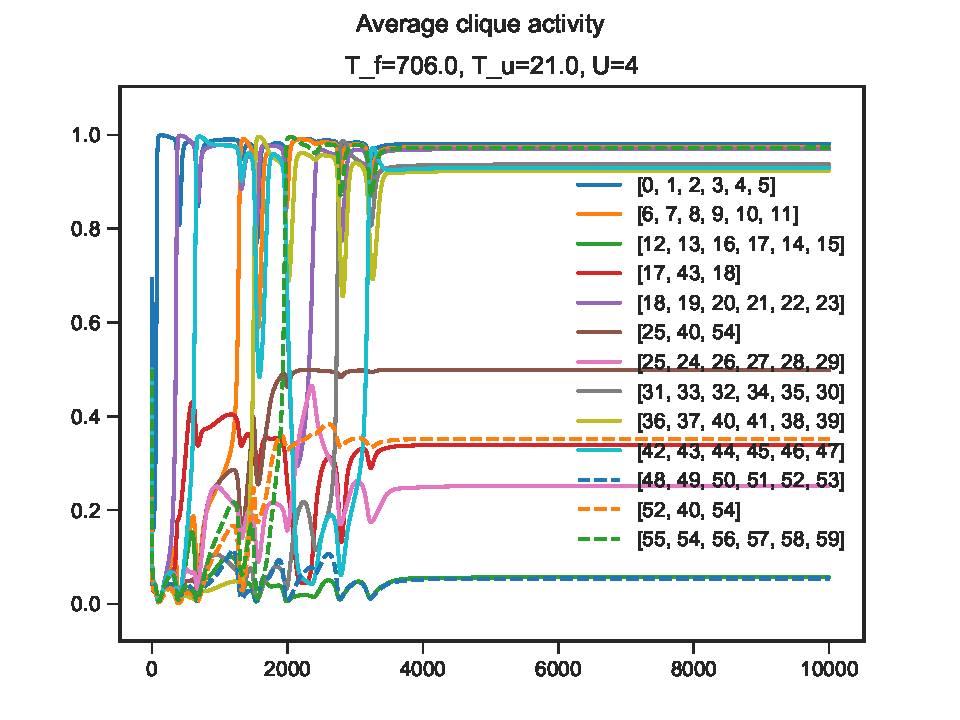
\includegraphics[width=.49\textwidth]{clique_activity_fix_notes}
		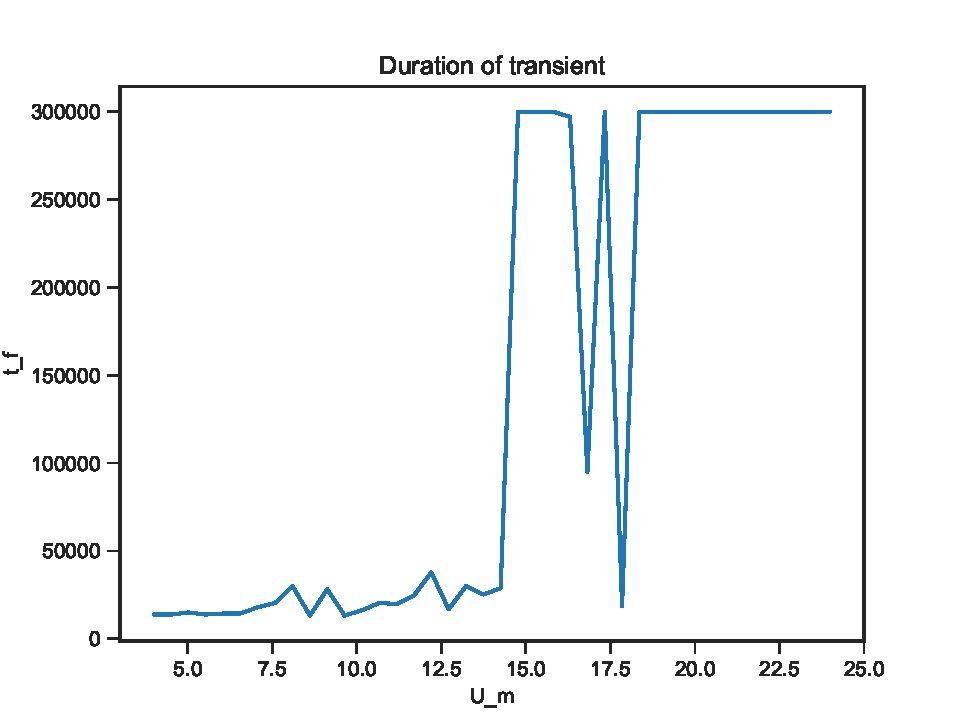
\includegraphics[width=.49\textwidth]{transient_duration.pdf}
		\caption{Left: The dynamics is characterized by fixpoints with $U=4$, $\tau_u=21\,\text{ms}$, $\tau_\varphi = 706\,\text{ms}$. Right: Duration of transient until a fixpoint is reached. As $U$ increases, an autonomous activity eventually takes over.}
		\label{fig:fixpoints}
	\end{figure}

	\begin{figure}
		\centering
		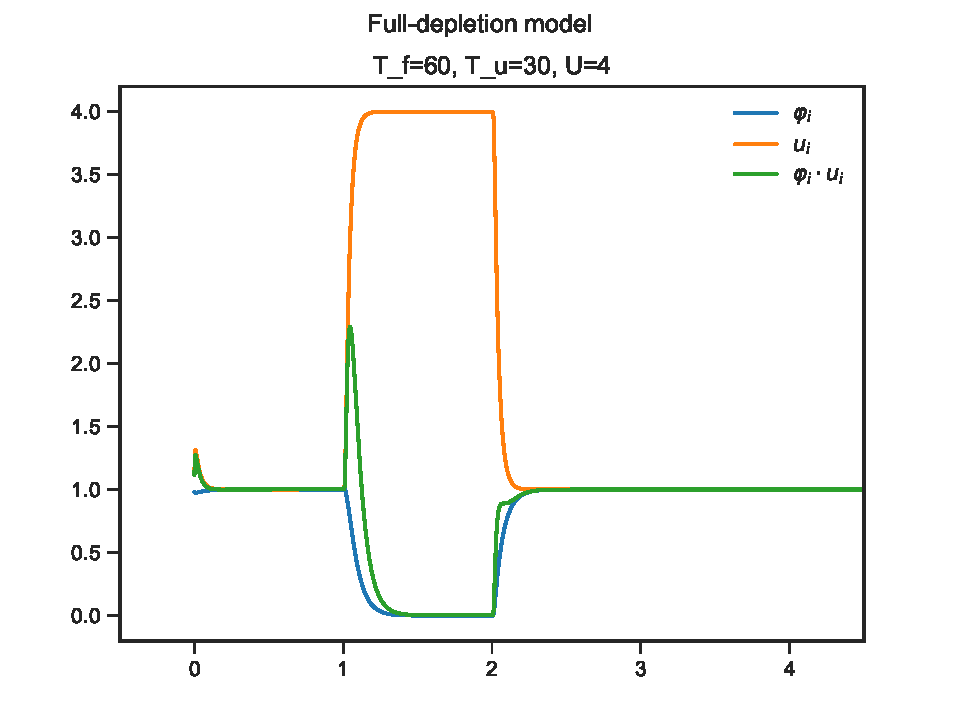
\includegraphics[width=.49\textwidth]{FD_standard}
		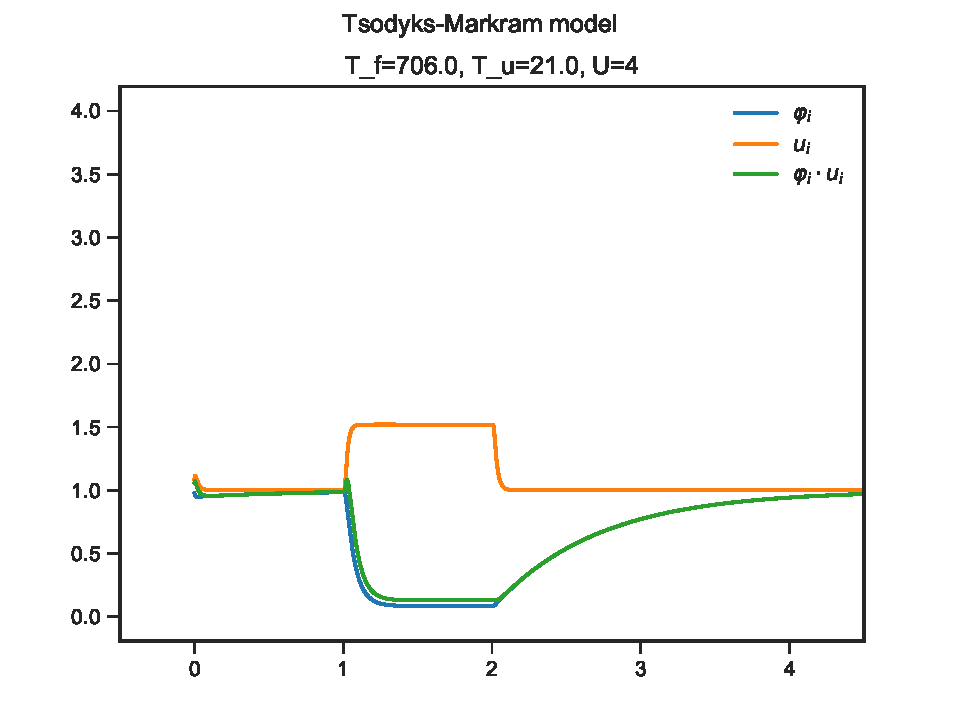
\includegraphics[width=.49\textwidth]{TM_notes}
		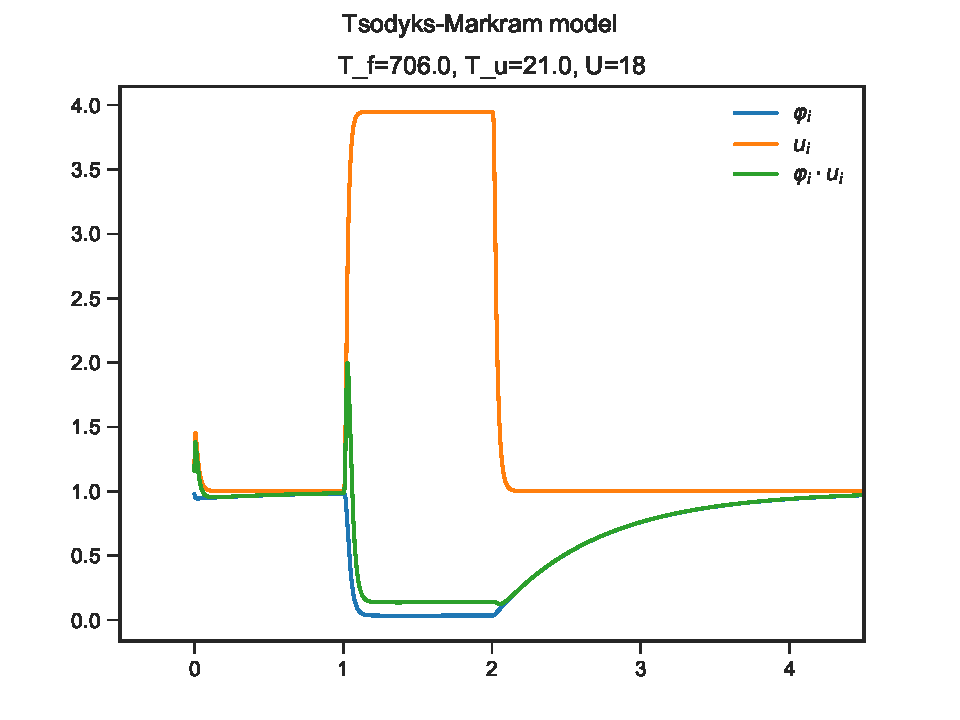
\includegraphics[width=.49\textwidth]{TM_U18}
		\caption{Top left: full depletion model used up to now. Top right: Tsodyks-Markram model from Gupta. Bottom: Tsodyks-Markram model with $U_m=18$.}
		\label{fig:two_stsp}
	\end{figure}
	
	Unfortunately a given value of $U_m$ does not ensure autonomous activity for networks with different number of cliques $n_c$, see Fig. \ref{fig:param_sweep}.
	
	\begin{figure}
		\centering
		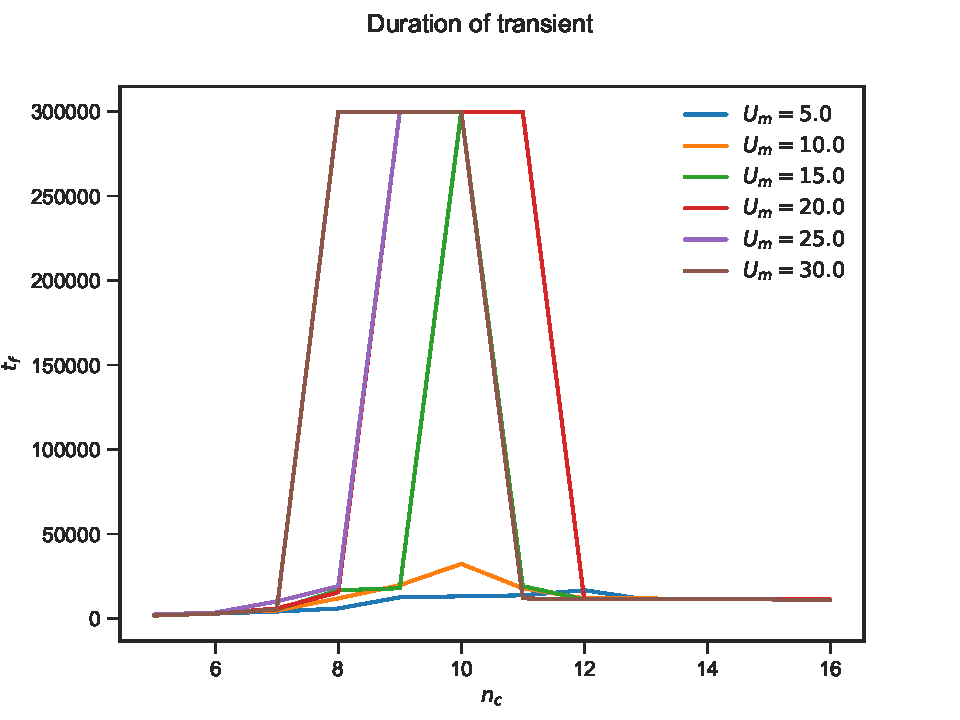
\includegraphics[width=.7\textwidth]{transient_sweep}
		\caption{}
		\label{fig:param_sweep}
	\end{figure}

\end{document}